\begin{pastexam}[label={px:nsysu-109-osds-02}]{中山資工所甲組 109 學年度 第 8 題}
（追蹤）

(5\%) Show the Huffman tree created from the following nodes arranged in a priority queue.
\begin{center}
\begin{tabular}{|c|c|c|c|c|c|c|c|c|c|}\hline
A & B & C & D & E & F & G & H & I & J\\
6 & 9 & 12 & 14 & 18 & 24 & 27 & 29 & 35 & 45\\\hline
\end{tabular}
\end{center}
\end{pastexam}

\begin{pastsoln}
霍夫曼演算法（資結書虛擬碼~19.3）：每次從優先佇列取出權重最小的兩棵樹，合併成一棵新樹（權重相加，先取出的
當左子樹），再放回佇列，做 $n - 1 = 9$ 次。
\begin{center}
\begin{tabular}{clll}
\toprule
次 & 取出的兩棵 & 新樹 & 合併後的佇列（權重） \\
\midrule
1 & A 6, B 9 & 15 & 12, 14, 15, 18, 24, 27, 29, 35, 45 \\
2 & C 12, D 14 & 26 & 15, 18, 24, 26, 27, 29, 35, 45 \\
3 & 15, E 18 & 33 & 24, 26, 27, 29, 33, 35, 45 \\
4 & F 24, 26 & 50 & 27, 29, 33, 35, 45, 50 \\
5 & G 27, H 29 & 56 & 33, 35, 45, 50, 56 \\
6 & 33, I 35 & 68 & 45, 50, 56, 68 \\
7 & J 45, 50 & 95 & 56, 68, 95 \\
8 & 56, 68 & 124 & 95, 124 \\
9 & 95, 124 & 219 & 219 \\
\bottomrule
\end{tabular}
\end{center}
過程中沒有兩個權重相同，所以每一步取哪兩棵是唯一的。 得到的霍夫曼樹（圓圈是合併出來的內部節點，方框是
葉子；左邊標 0、右邊標 1）：
\begin{center}
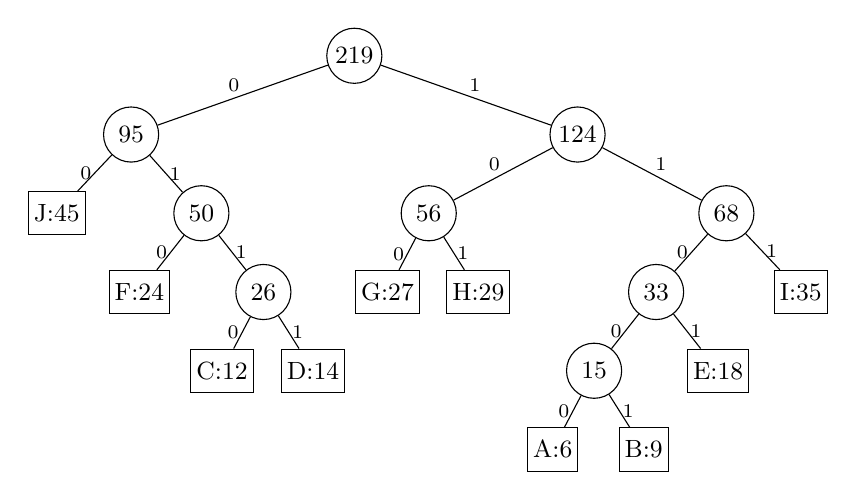
\begin{tikzpicture}[x=1.05cm,y=1.0cm,
  inn/.style={circle,draw,inner sep=1pt,minimum size=7mm,font=\small},
  lf/.style={rectangle,draw,inner sep=2pt,minimum height=5.5mm,font=\small},
  b/.style={font=\scriptsize,inner sep=1pt}]
\node[inn] (r) at (3.6,0) {219};
\node[inn] (n95) at (0.9,-1) {95};
\node[inn] (n124) at (6.3,-1) {124};
\node[lf] (J) at (0,-2) {J:45};
\node[inn] (n50) at (1.75,-2) {50};
\node[inn] (n56) at (4.5,-2) {56};
\node[inn] (n68) at (8.1,-2) {68};
\node[lf] (F) at (1,-3) {F:24};
\node[inn] (n26) at (2.5,-3) {26};
\node[lf] (G) at (4,-3) {G:27};
\node[lf] (H) at (5.1,-3) {H:29};
\node[inn] (n33) at (7.25,-3) {33};
\node[lf] (I) at (9,-3) {I:35};
\node[lf] (C) at (2,-4) {C:12};
\node[lf] (D) at (3.1,-4) {D:14};
\node[inn] (n15) at (6.5,-4) {15};
\node[lf] (E) at (8,-4) {E:18};
\node[lf] (A) at (6,-5) {A:6};
\node[lf] (B) at (7.1,-5) {B:9};
\draw (r)--node[b,above left]{0}(n95); \draw (r)--node[b,above right]{1}(n124);
\draw (n95)--node[b,left]{0}(J); \draw (n95)--node[b,right]{1}(n50);
\draw (n124)--node[b,above left]{0}(n56); \draw (n124)--node[b,above right]{1}(n68);
\draw (n50)--node[b,left]{0}(F); \draw (n50)--node[b,right]{1}(n26);
\draw (n56)--node[b,left]{0}(G); \draw (n56)--node[b,right]{1}(H);
\draw (n68)--node[b,left]{0}(n33); \draw (n68)--node[b,right]{1}(I);
\draw (n26)--node[b,left]{0}(C); \draw (n26)--node[b,right]{1}(D);
\draw (n33)--node[b,left]{0}(n15); \draw (n33)--node[b,right]{1}(E);
\draw (n15)--node[b,left]{0}(A); \draw (n15)--node[b,right]{1}(B);
\end{tikzpicture}
\end{center}
對應的編碼：J \texttt{00}，F \texttt{010}，C \texttt{0110}，D \texttt{0111}，G \texttt{100}，H \texttt{101}，
A \texttt{11000}，B \texttt{11001}，E \texttt{1101}，I \texttt{111}。 加權路徑長（每個字元的權重乘上編碼長度）：
\[
45 \cdot 2 + (24 + 27 + 29 + 35) \cdot 3 + (12 + 14 + 18) \cdot 4 + (6 + 9) \cdot 5 = 90 + 345 + 176 + 75 = 686,
\]
也等於所有內部節點的權重和 $15 + 26 + 33 + 50 + 56 + 68 + 95 + 124 + 219 = 686$。

左右怎麼擺沒有規定，兩個子樹左右對調得到的樹一樣是霍夫曼樹，編碼長度不變；作答時畫一棵、寫清楚合併順序即可。
\end{pastsoln}
